% !TEX root = ../thesis_main.tex



%%%% --- * --- %%%%
\clearpage	
\chapter{Estimating Systematic Effects}
\label{systematics_chapter}
	\note{How do I even \emph{do} these estimations?}
	\section{Low-energy Scintillator Threshold}
	%\\*
	Choice of low-energy scintillator threshold has a large systematic effect...  \aside{It's actually not nearly as big as I'd originally expected.  It's huge in the lineshape thing, but pretty tiny in everything else.}
	
	\section{BB1 Radius, Energy Threshold, Agreement}
	\label{section:bb1_systematics}
	%\\*
	BB1 radius cut can help to eliminate scattered events.  Energy threshold selection and statistical agreement between BB1 detectors' energies only makes a small effect on results.  BB1 radius itself has a pretty big effect on the result, but we can at least just G4 it away.  The remaining systematic effect is pretty small.
	\note[color=jb]{As per JB's comment in section~\ref{thesisconventionjb}:   ``statistical agreement between BB1 X and Y detectors' energies only makes a small effect on results" does not need the technical details beyond that statement."}
	
\missingfigure{Surely this requires at *least* one image of the pixelated BB1 data.  Maybe some of a few waveforms and energy distributions too.  ....Feels like cheating to include some of that stuff, since Ben was the one who actually used it mostly.}

\note{Remember:  There's noise applied to simulated BB1s, matching some spectrum.}
In the end, we get our results from the scintillator energy only, without summing the BB1 energy back in.  Energy absorbed in DSSDs is only used as (a) a tag for events, and (b) contributing to the total beta energy loss before the beta arrives at the scintillator.


\section{Background Modeling -- Decay from Surfaces within the Chamber}
	So many surfaces, all of which can get stray 37K atoms stuck to them.  Then they decay from a place that isn't the actual trap center, and it contaminates our stuff.
	
%	\missingfigure{Show modelled TOF spectra in comparison with real TOF spectra.  Show the cut we made on that. }
	\missingfigure{Show the "average asymmetry" (all energies) as a function of TOF, with real data, best model normalization, and extrema of model normalizations.  Show our cut.  Turns out, it's a lot of work for a really tiny correction.  Oh well.}
	
	So we model the beta TOF from the surfaces in G4, event by event.  This is necessary because scattered events will have their TOF changed to account for a longer beta pathlength, and we're preferrentially cutting away the events that don't have a TOF in the appropriate range.  ....And then have COMSOL generate electron TOFs for SOEs starting from the start points picked by G4.  Ran COMSOL for 0 eV SOEs, and again for Levinger spectrum SOEs.  Used ~9\% 0eV SOEs in the end.  I forget which Levinger distribution I used in the end.  The point is, for each event, you've simulated a beta TOF that may or may not be scattered off of something before it hits a detector, and you have a SOE TOF for an event originating at that same point, so you subtract them to model the TOF you'd measure in an experiment.  Also, because you've done the scattering with G4, you get the beta energy corrected for any scattering that happened.  This way, you know precisely how much "bad stuff" you're getting rid of with the TOF cut.
	
%	\subsection{Decay from Chamber Surfaces}

\section{Quantifying the Effects Backscatter with Geant4}
	Beta decay (back-)scatter from surfaces within the experimental chamber is a significant systematic, and it must be evaluated, quantified, and corrected for.  This is done via a series of GEANT4 simulations.  While only a small fraction of events are affected, the process results in an energy loss in the beta that can, if not understood, be misinterpreted as the exact signal we're searching for.  It is therefore imperative that this be well understood. 
	\aside{Oh god.  Have I even \emph{tried} to quantify the combined systematic that comes out of the TOF cut?  Do I need to, or is it double-counting?  Ugh, it would be such a headache to do this.  Maybe I can at least do it at the end -- because I might never get my code back to the way it was.}


%	\missingfigure{Show simulated $\cos\theta$ vs TOF.  You can just make a lot of that go away with a properly selected cut.}
\begin{figure}[h!!!t]
	\centering
	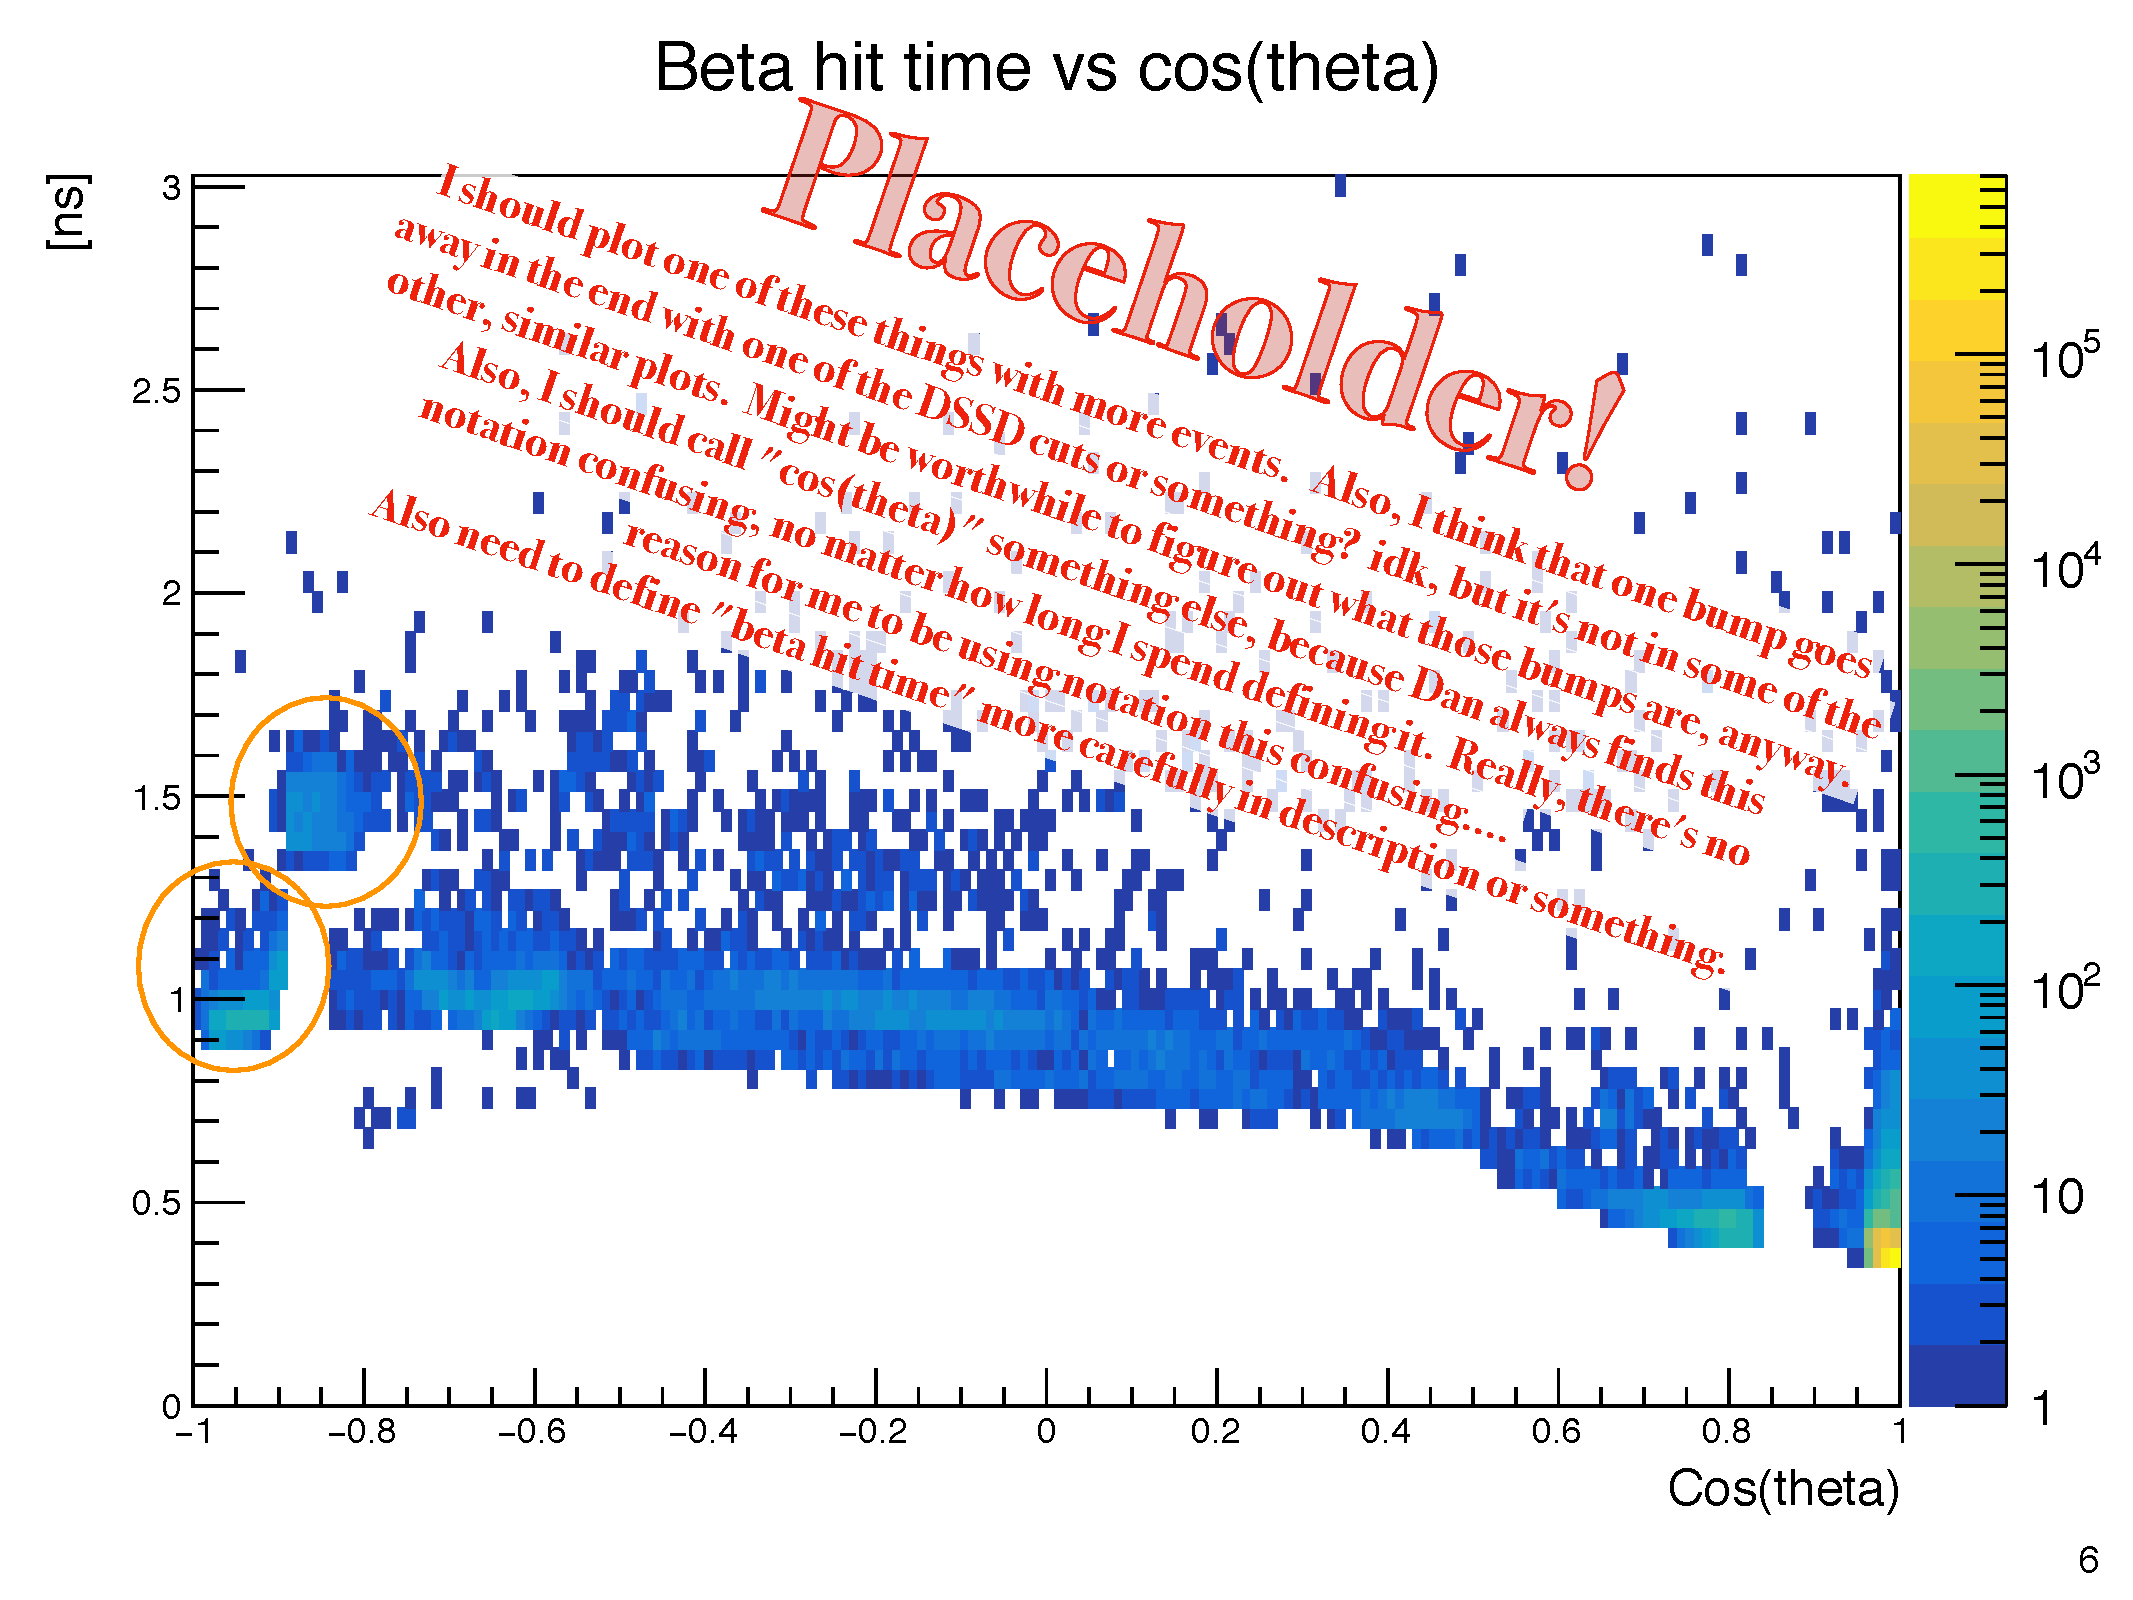
\includegraphics[width=.999\linewidth]
	{Figures/toa_vs_costheta.pdf}
	\caption[Simulated Beta TOA vs emission angle w.r.t. detector orientation]{Simulated Beta TOA vs emission angle w.r.t. detector orientation}	
	\label{fig:toa_vs_costheta}
\end{figure}


\section{Lineshape Reconstruction}
	\note[color=jb]{This section should reference Clifford.~\cite{clifford}.}
	\subsection{Motivation}
	This process is used because the (back-)scatter, which it itself an important systematic, is largely independent of a wide variety of other experimental effects.  These other effects must all be evaluated, but it is computationally prohibitive to re-evaluate the scattering with every other effect under consideration.
	
	\subsection{What is it and how does it work?}
	Mono-energetic beta decay events are generated in GEANT4, which outputs an energy spectrum for unscattered and forward-scattered beta events in the detector.  These spectra are fit to a function to model the scintillator resolution, as well as energy loss in materials that the beta passed through before arriving at the scintillator.  These spectrum fits are performed for a set of beta energies, and parameters are extrapolated to be applied to betas emitted at intermediate energies.  Thus, the whole spectrum can be modeled.  Pictures will make this clearer. 
	
	\subsection{The Math-Specifics}
	I'll write down the specific functions I'm using, and the parameter values I'm using.  (Maybe this should go in an appendix instead?)  I'll describe the adjustments I make to the spectrum so that it can work even for the dataset where the scintillators' resolutions have changed.
	
	\subsection{The Results -- Things That Got Evaluated This Way}
	As it turns out, only cloud parameters were evaluated this way.  Trap position, size, sail velocity, temperature.  But then we varied the lineshape anyhow, to account for G4 doing a bad job of modelling the bremsstrahlung (sp?).
	%Thicknesses of the SiC mirror, the Be foil, and the DSSD.  Scintillator calibration.  
	
	\subsection{The low-energy tail uncertainty, and what it does}
	Bremsstrahlung.  It does Bremsstrahlung.

